% !TEX TS-program = pdflatexmk
\documentclass[12pt]{article}
\usepackage{float}

\usepackage{amsthm}

% Layout.
\usepackage[top=.75in, bottom=0.75in, left=.75in, right=.75in, headheight=1in, headsep=6pt]{geometry}

\usepackage{fancyhdr, enumerate,multirow}
% Fonts.
\usepackage{mathptmx}
\usepackage[scaled=0.86]{helvet}
\renewcommand{\emph}[1]{\textsf{\textbf{#1}}}

% Misc packages.
\usepackage{amsmath,amssymb,latexsym}
\usepackage{graphicx,tikz}
\usepackage{array}
\usepackage{xcolor}
\usepackage{multicol}
\usepackage{tabularx,colortbl}
\usepackage[T1]{fontenc}
\usepackage{enumitem}
%to make tikz pics work
\usepackage{tikz,pgfplots}

\usepackage{varwidth}
\usepackage{verbatim}
\usepackage{mathtools}
\DeclarePairedDelimiter\ceil{\lceil}{\rceil}
\DeclarePairedDelimiter\floor{\lfloor}{\rfloor}

\newenvironment{centerverbatim}{%
  \par
  \centering
  \varwidth{\linewidth}%
  \verbatim
}{%
  \endverbatim
  \endvarwidth
  \par
}

\makeatletter
\newenvironment{centeredverbatim}{\expandafter\verbatim\centering}{\endverbatim}
\makeatother


\usetikzlibrary{arrows}
\newcommand{\midarrow}{\tikz \draw[-triangle 90] (0,0) -- +(.1,0);}

\usepackage[colorlinks=true]{hyperref}

% Paragraph spacing
\parindent 0pt
\parskip 6pt plus 1pt
\def\tableindent{\hskip 0.5 in}
\def\ts{\hskip 1.5 em}

\usepackage{fancyhdr}
\pagestyle{fancy} 
\lhead{\large\sf\textbf{MATH 663 }}
\rhead{\large\sf\textbf{Fall 2023}}
\chead{\large\sf\textbf{HW 10}}

\newcommand{\localhead}[1]{\par\smallskip\textbf{#1}\nobreak\\}%
\def\heading#1{\localhead{\large\emph{#1}}}
\def\subheading#1{\localhead{\emph{#1}}}

%% Special Math Symbol shortcuts
\newcommand{\NN}{\mathbb{N}}
\newcommand{\RR}{\mathbb{R}}

\newcommand{\rad}{\text{rad}}
\newcommand{\diam}{\text{diam}}
\newcommand\solution{\localhead{Solution:}}

%\newenvironment{clist}%
%{\bgroup\parskip 0pt\begin{list}{$\bullet$}{\partopsep 4pt\topsep 0pt\itemsep -2pt}}%
%{\end{list}\egroup}%

\usetikzlibrary{calc,arrows.meta}
%\pgfplotsset{my style/.append style={axis x line=middle, axis y line=
%middle, xlabel={$x$}, ylabel={$y$}, axis equal }}{





\usetikzlibrary{calc,arrows.meta}
%\pgfplotsset{my style/.append style={axis x line=middle, axis y line=
%middle, xlabel={$x$}, ylabel={$y$}, axis equal }}
\usetikzlibrary{arrows}
\newcommand{\marrow}{\tikz \draw[-triangle 90] (0,0) -- +(.1,0);}


\begin{document}
\begin{enumerate}
	\item Let $m,n \in \mathbb{N},$ and assume that $m-1$ divides $n-1.$ Show that every tree $T$, of order $m$ satisfies $R(T,K_{1,n})=m+n-1.$
	\begin{proof} 
		Let $m,n \in \mathbb{N},$ and assume that $m-1$ divides $n-1$. So $(m - 1)J = (n - 1)$ for some $J \in \NN$. Note that, 
		\begin{equation*}
			(J + 1)(m - 1) = \left(\frac{(n - 1)}{(m- 2)} + 1\right)(m - 1) = (n - 1) + (m - 1) = n + m - 2
		\end{equation*}
		Construct a complete graph $K^{m + n - 2}$ by $J + 1$ copies of red $K^{m - 1}$ to avoid $T$. Let $v$ be some vertex, and note that by construction it must have $J(m - 1) = n - 1$ incident blue edges since there are $J$ copies of $k^{m - 1}$ which we must connect to $v$ via blue edges, so by construction we avoid a $K_{1, n}$. Hence $R(T, K_{1, n}) > m + n - 2$ \\



		

		Suppose $T$ is a tree with order $M$, and consider some edge 2-coloring of $K^{m + n - 1}$. Suppose there does not exists a blue $K_{1, n}$. Note that every vertex has $m + n - 2$ incident edges. Let $v$ be a vertex and note that $v$ must have strictly less than $n - 1$ incident blue edges, and therefore $v$ must have strictly more than $m + n - 2 - n + 2 = m - 1$ incident red edges. Now clearly the red coloring of $K^{m + n - 1}$ forms a subgraph $H$ such that $\delta(H) \geq m - 1$. By Corollary 1.5.4 we find that $T \subset H$.\\

	




	\end{proof}
	\newpage







	\item Prove that $R(3,4)=R(K^3,K^4)=9.$ (Proof from Mazur) 
	
	\begin{proof} Consider a $K^{9}$ with some edge 2-coloring. First note that the subgraph induced by the red edges, of course has an odd number of vertices, and therefore there must be a vertex of even degree. Let $v \in K^9$ with an even number of incident red edges. Now consider two cases: \\

		There are least 3 or more red edges incident to $v$, in which case $v$ has at least 4 incident red edges. Consider the $K^4$ induced by 4 neighbors of $v$ adjacent by red edges. Since $R(K^2, K^4) = 4$ then such a $K^4$ is either blue, in which case we are done, or it contains a red $K^2$. Such a red $K^2$ would form a red $K^3$ with $v$.\\


		There are at most two red edges incident to $v$, in which case there are at least 6 incident blue edges. Consider the $K^6$ induced by 6 neighbors of $v$ adjacent by blue edges. Since $R(K^3, K^3) = 6$, then such a $K^6$ contains either a red $K^3$ in which case we are done, or a blue $K^3$. Such a blue $K^3$ would form a blue $K^4$ with $v$.
		\begin{figure}[H]
			\begin{center}
				\caption{Counter example for $R(3, 4) > 8$}
				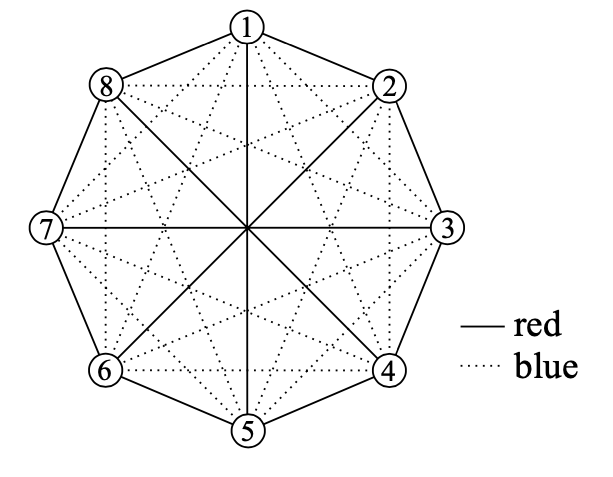
\includegraphics[width=.45\textwidth]{CounterExample.png}
			\end{center}
		\end{figure}
	\end{proof}
	\newpage


	\item An oriented complete graph is called a tournament. A Hamilton path is a path through every vertex of the graph. Show that every tournament contains a directed Hamilton path. 
	\begin{proof} We will proceed by induction on the number of vertices $n$, in our tournament $T$. The base case is trivial, $n = 1$ the statement hold vacuously and $n = 2$ the only path to choose from is a Hamilton path. 

		Suppose we have a tournament, $T$ on $n + 1$ vertices. Consider a vertex $v$ and note by the induction hypothesis there exists a length $n$ hamiltonian path in $T \setminus v$, we'll call it $v_0, v_1, v_2, \dots v_n$. Now consider two cases: 
		
		every arc incident to $v$ is of the form $(v, v_i)$ or $(v_i, v)$, in which case $v$ can be added to the beginning or end of induced hamiltonian path to form a new hamiltonian path on $T$. 
		
		There exists both types of arcs $(v, v_i)$ or $(v_i, v)$ incident to vertex $v$. Now consider the arc of the form $(v_{j}, v)$ with maximal $j$. If $j = n$ then we append $v$ to the induced hamiltonian path and from a new hamiltonian path for $T$. Otherwise there must exists an arc of the form $(v, v_{j + 1})$, in which case we form the following hamiltonian path on $T$, 
		\begin{equation*}
			v_0, \dots v_j, v, v_{j + 1}, \dots v_n. 
		\end{equation*}
	\end{proof}
	\newpage
	
	
	\item Show that every uniquely 3-edge-colorable cubic graph is hamiltonian. By \emph{uniquely} 3-edge-colorable, we mean that every 3-edge coloring induces the same edge partition.
	\begin{proof} Suppose $G$ is a uniquely 3-edge-colorable cubic graph. By definition the  3-edge coloring induces an edge partition, into 3 parts $E_1$, $E_2$, and  $E_3$. Now since $G$ is 3-regular each $E_i$ must forms a one-factor. Note that $E_1 \cup E_2$ is a graph of disjoint even cycles. Consider creating a path starting at $v$, note it must alternate $E_1, E_2$ edges, since the larger graph is cubic, such a path must terminate at $v$ via a free edge forming a cycle. This cycle is either contains every vertex in the graph, or it doesn't, in the case that it doesn't the rest of the vertices must lie on a similar even cycle. 

		Now should $E_1 \cup E_2$ form a hamiltonian cycle, we are done. If they do not then there exists an even cycle $C \subset E_1 \cup E_2$ for which we can swap edges and form a new edge partition, which is distinct from our original partition, a contradiction. 
 		
	\end{proof}
 

	\newpage
	
	
	\item 
	\begin{enumerate}
	\item Prove Ore's Lemma stated below:
	\begin{quote} Let $G$ be a graph on $n$ vertices. If $u$ and $v$ are distinct nonadjacent vertices in $G$ such that $d(u)+d(v)\geq n,$ then $G$ is hamiltonian if and only if $G+uv$ is hamiltonian.\end{quote}
	\begin{proof} The forward direction is trivial, if $G$ is hamiltonian, then $G + e$ any edge will still be hamiltonian, via the same hamiltonian cycle on $G$.  
	\end{proof}
	\begin{proof} Suppose $G$ is graph on $n$ vertices let $u$ and $v$ are distinct nonadjacent vertices in $G$ such that $d(u)+d(v)\geq n$ and suppose $G + uv$ is hamiltonian. Clearly if a hamiltonian cycle on $G + uv$ fails to use edge $uv$ then we have a hamiltonian cycle on $G$ in which case we are done. Now let $C$ be a hamiltonian cycle on $G + uv$ which contains the edge $uv$. Let $uPv$ be the hamiltonian path which excludes $uv$, and therefore $P \subseteq U$.  Since $d(u) + d(v) \geq n$ suppose without loss of generality that $d(u) \geq \frac{n}{2}$. If for some $p_i \in P$, there exists $vp_{i - 1}$ and $up_{i}$ then we can form a hamiltonian cycle in $G$ (We have seen this reasoning before). Counting the set of vertices which do not form such a hamiltonian cycle, 
		\begin{equation*}
			\underbrace{\underbrace{(n - 2)}_{\text{\# of possible neighbors}} - \underbrace{d(u)}_{\text{number of vertices 'behind' a neighbor of $u$}}}_{\text{\# of bad vertices which don't produce a hamiltonian cycle when incident to $v$}}. 
		\end{equation*}
		Now clearly it follows by our hypothesis that, 
		\begin{align*}
			d(u) + d(v) &\geq (n - 2)\\
			d(v) &\geq (n - 2) - d(u)\\
		\end{align*}
		So $u$ and $v$ must have neighbors in $P$ which produce a hamiltonian cycle in $G$.
	\end{proof}








	\item Use Ore's Lemma to prove that if $G$ is a graph on $n$ vertices such that $d(u)+d(v) \geq n$ for all nonadjacent vertices, then $G$ is hamiltonian.
	\begin{proof} Suppose $G$ is a graph on $n$ vertices such that $d(u)+d(v) \geq n$ for all nonadjacent vertices and for the sake of contradiction suppose $G$ is not hamiltonian. Suppose we add edges to form $G'$ a maximally a-hamiltonian graph. Thus $G' + uv$ is hamiltonian and by the reverse direction of Ore's Lemma $G'$ is also hamiltonian, a contradiction. 
	\end{proof}






	\item Show that the hypothesis in part (b) is weaker than the hypothesis in Dirac's Theorem.
	\end{enumerate}
	\begin{proof} Suppose a graph $G$ with $n \geq 3$ vertices and $\delta(G) \geq \frac{n}{2}$. Well clearly for any pair of vertices $u, v$ (not just the non adjacent ones) we have that, 
	\begin{equation*}
		d(u) + d(v) \geq \delta(G) + \delta(G) = n.
	\end{equation*}
	\end{proof}
	\newpage
	
	
	
	\item Show that a connected graph $G$ is countable if all its vertices have countable degrees.
	\begin{proof} Let $G$ be a connected graph, such that all its vertices have countable degrees.Let $v \in G$ and consider the following, recursive union of neighborhoods
		\begin{align*}
			N_1 = \{v\},\\
			N_2 = \{N(v)\},\\
			N_3 = \{N(N_2) \setminus N_2\},\\
			N_i = \{N(N_{i - 1}) \setminus N_{i - 1}\},\\
		\end{align*}
		\begin{equation*}
			N^* = \bigcup_{i = 1}^\infty N_i
		\end{equation*}
		Clearly $N^* \subseteq V$, and we assert $N^* \supseteq V$ and that that $N^*$ is countable. Note that for all $u \in G$ there exists a finite, length  $n$ path between $v$ and $u$, in which case we can be certain that $u \in N_n$ and hence $N^* \supseteq V$, so $|V| = |N^*|$. Note that, $N^*$ is a countable union of countable sets and is therefore countable. Hence $G$ is countable. 
	\end{proof}
	\newpage
	
	
	
	
	
	\item Let $G$ be an infinite graph and $A,B \subseteq V(G).$ Show that if no finite set of vertices separates $A$ from $B$ in $G$, then $G$ contains an infinite set of disjoint $A$-$B$ paths.
	\begin{proof} By Theorem 8.4.2 we know that $G$ contains a set of $\mathcal{P}$ disjoint $A-B$ paths and an $A-B$ separator on $\mathcal{P}$. (I have skimmed the discussion about this Theorem and recognize that it is not a trivial thing to cite, Menger's Theorem does not easily apply to infinite graphs).

	Now by our hypothesis we know that the $A-B$ separator on $G$ is not finite, and therefore $\mathcal{P}$ must contain an infinite number of paths. 
		
	\end{proof}
	






\end{enumerate}
\end{document}